\subsection{Transportation}
\begin{frame}
\frametitle{Fuel demand}
\begin{columns}
    \column[t]{5cm}
	\begin{figure}[htbp!]
		\begin{center}
			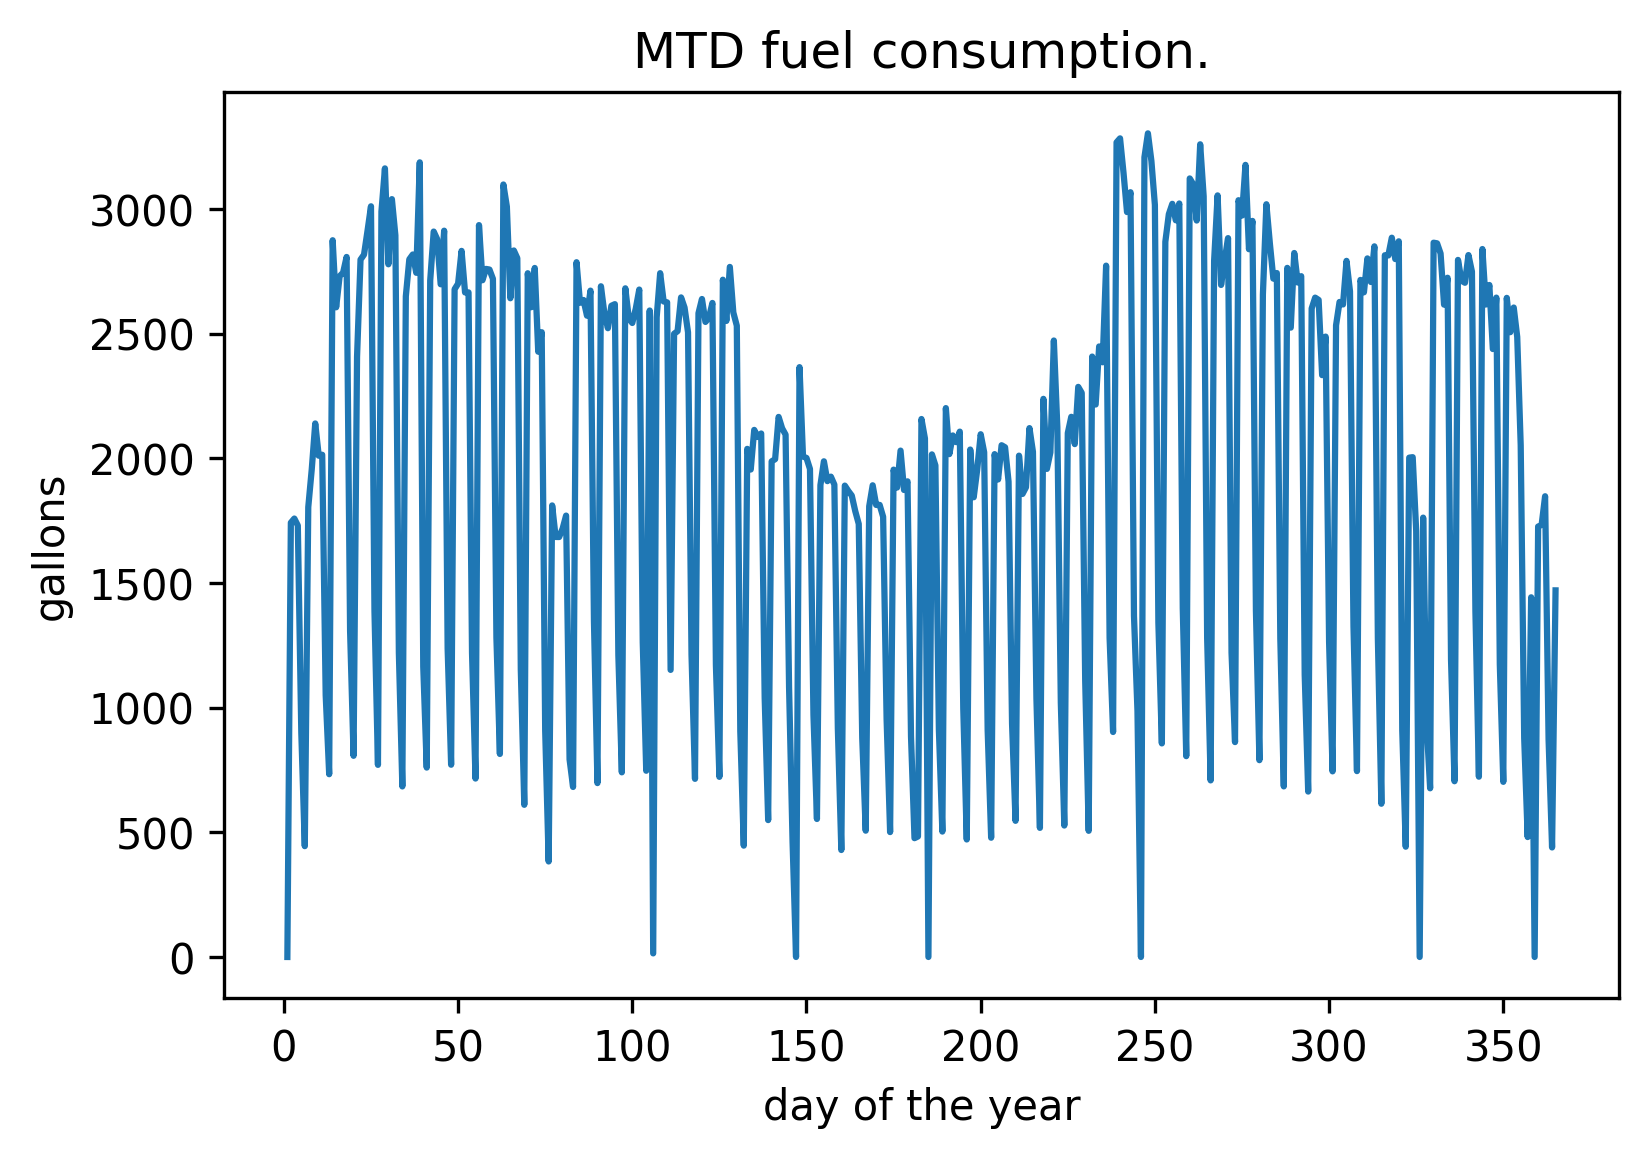
\includegraphics[height=4cm]{images/mtd2}
		\end{center}
		\caption{MTD fuel consumption. Data goes from July 1, 2018, until June 30, 2019 \cite{mtd_irecords_2019}.}
	\end{figure}

	\column[t]{5cm}
	\begin{figure}[htbp!]
		\begin{center}
			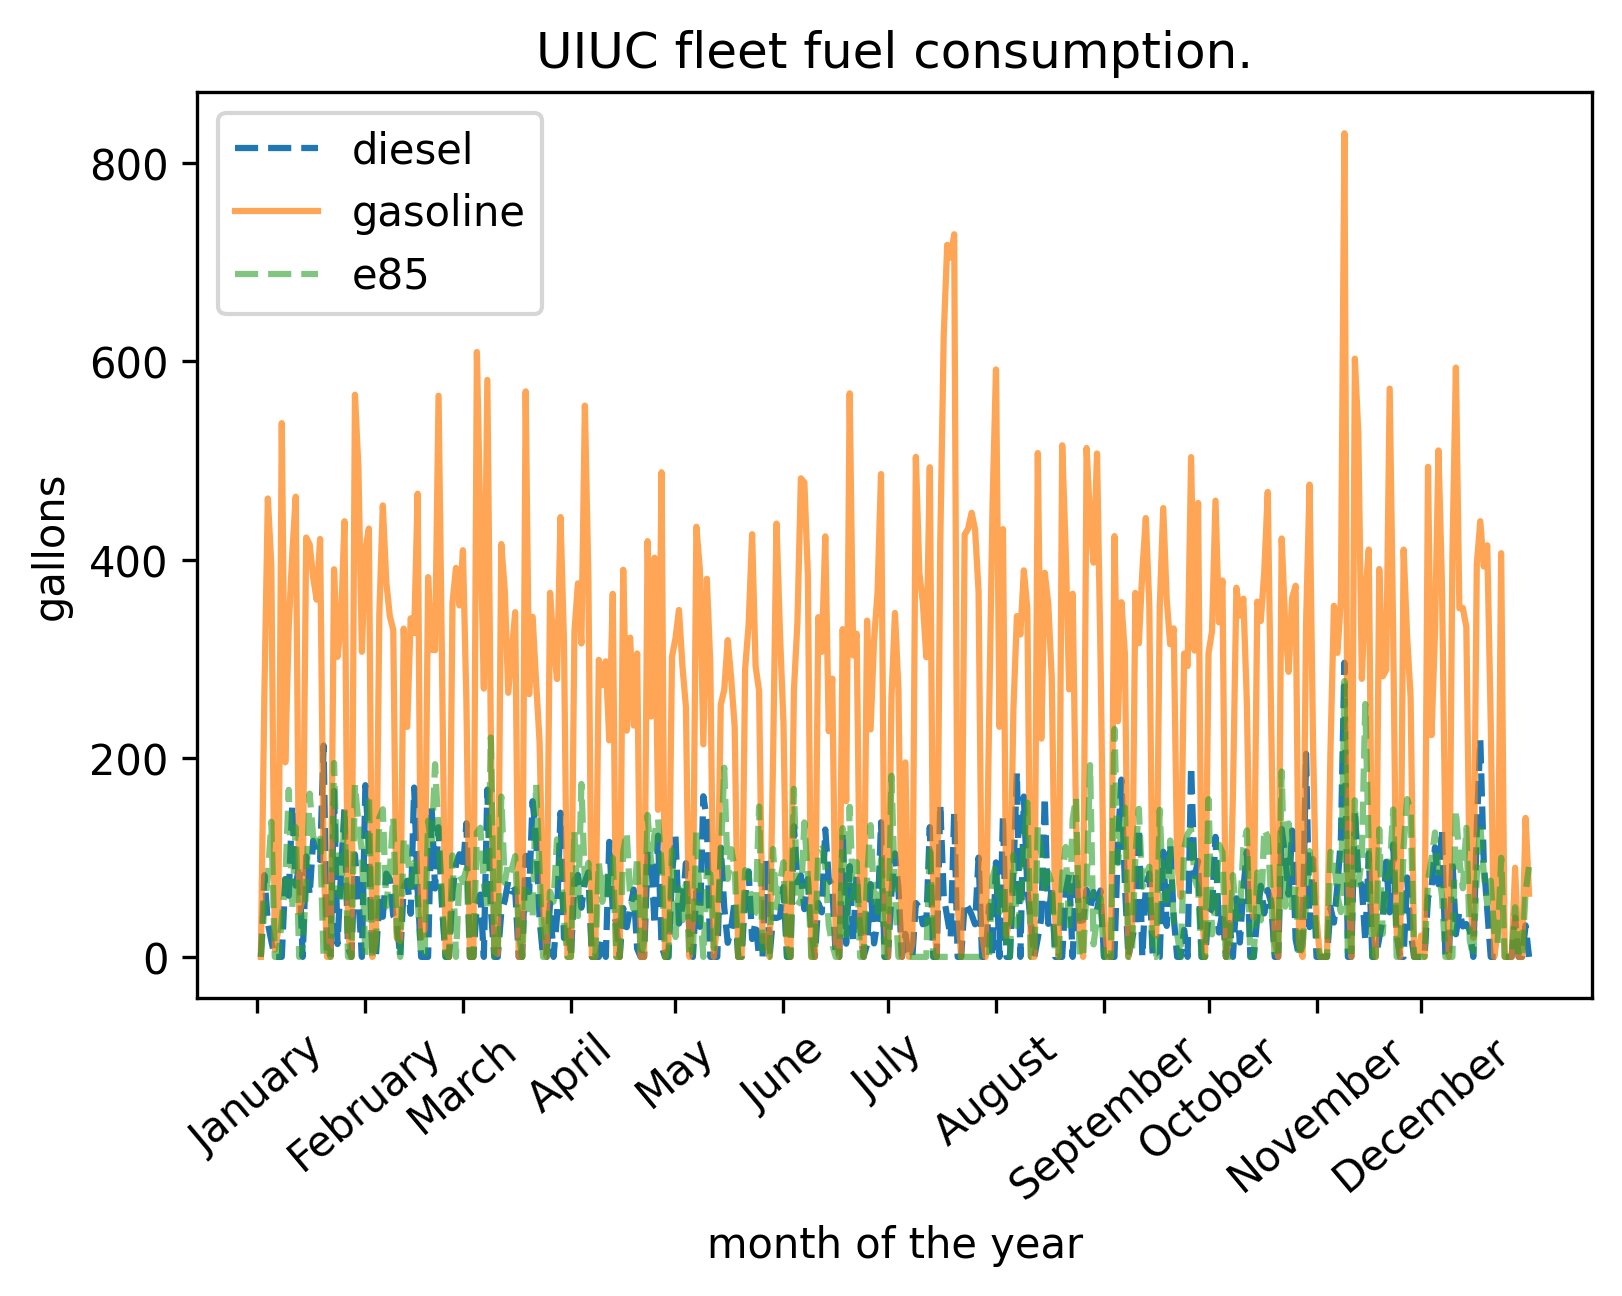
\includegraphics[height=4cm]{images/uiuc}
		\end{center}
		\caption{UIUC fleet fuel consumption. Data goes from January 1, 2019, until December 31, 2019 \cite{uiuc_personnal_communication}.}
	\end{figure}
\end{columns}
\end{frame}


\begin{frame}
\frametitle{Hydrogen requirement}
\begin{columns}
    \column[t]{5cm}
	\begin{table}[!htb]
		\centering
	    \caption{GGE, DGE, and E85GE \cite{doe_office_of_energy_efficiency_and_renewable_energy_hydrogen_2020} \cite{alternative_fuels_data_center_fuel_2014}.}
		\begin{tabular}{l|l}
		\hline
		                 & Hydrogen \\ \hline
		GGE              & 1 kg     \\
		DGE              & 1.13 kg  \\
		E85GE            & 0.78 kg  \\ \hline
        \end{tabular}
	\end{table}

	\begin{table}[!htb]
		\centering
	    \caption{Hydrogen requirements.}
		\begin{tabular}{l|l}
		\hline
		Total [tonnes/year]  & 943      \\
		Average [kg/day] 	 & 2584     \\
		Average [kg/h] 		 & 108      \\
		Maximum in one day   & 4440 kg  \\ \hline
        \end{tabular}
	\end{table}

	\column[t]{5cm}
	\begin{figure}[htbp!]
		\begin{center}
			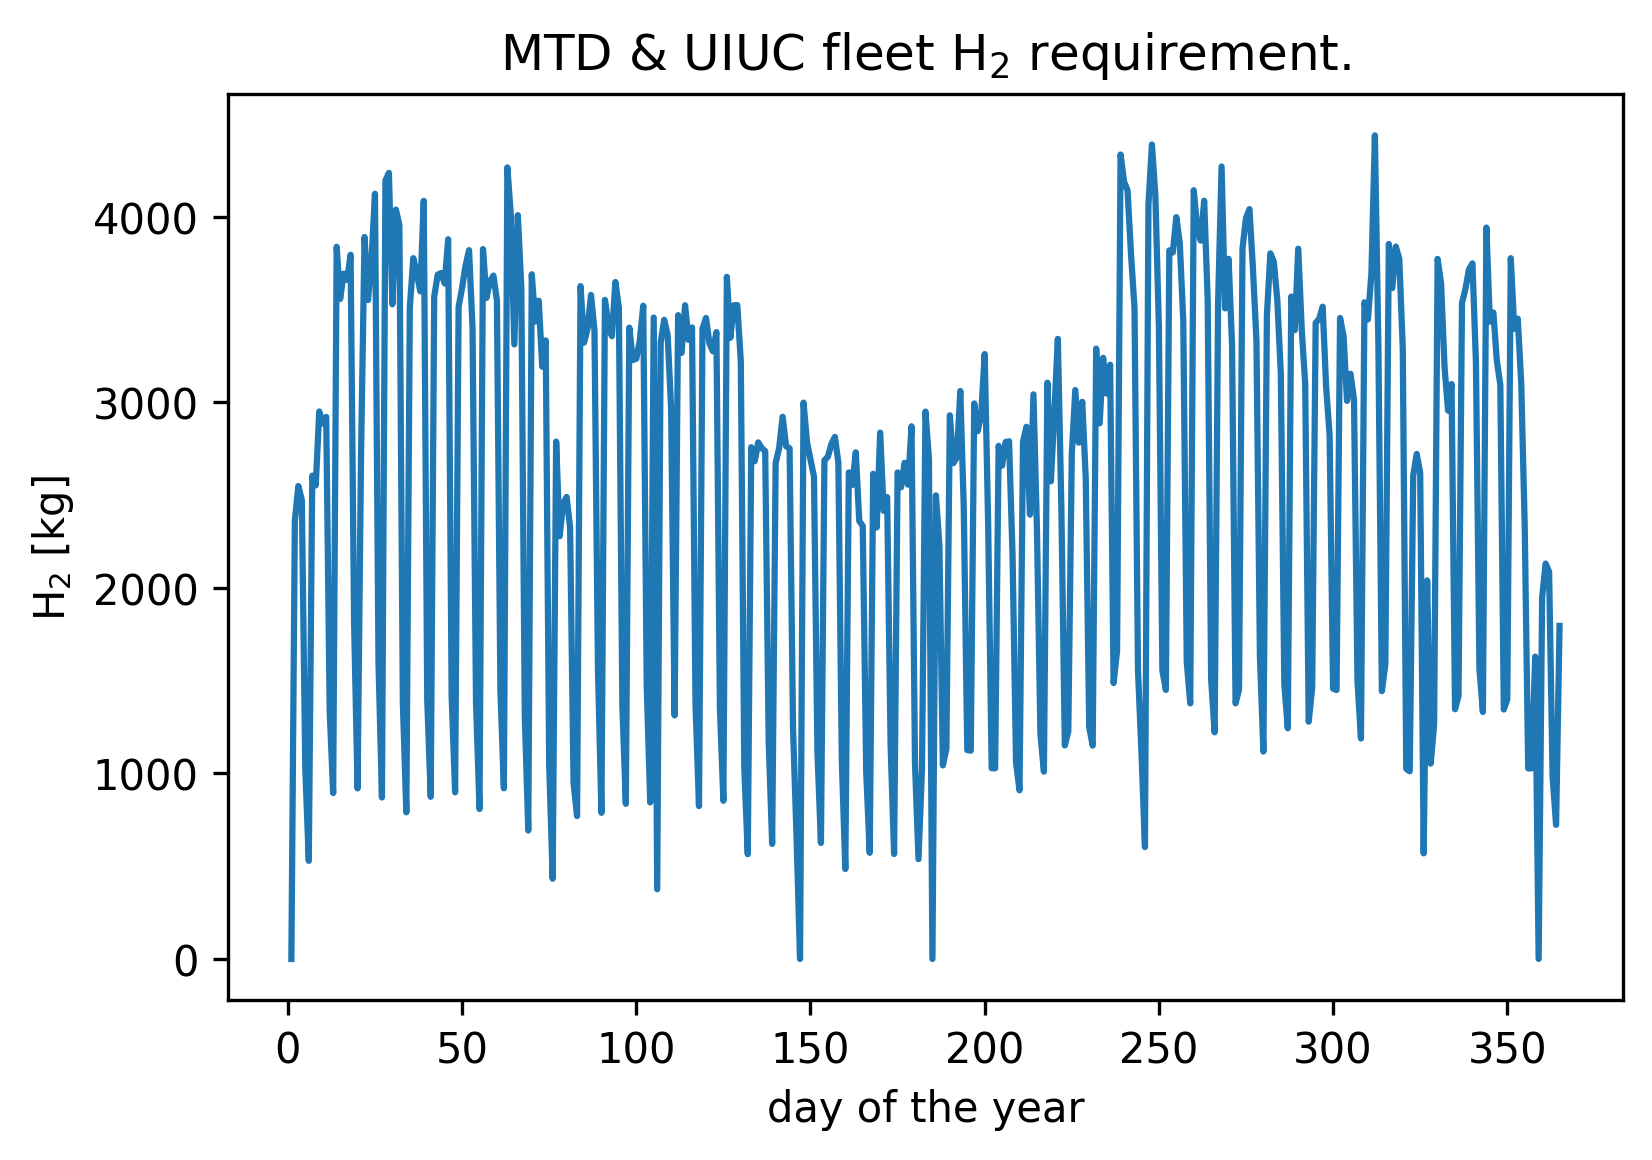
\includegraphics[height=4.3cm]{images/hydro-fleet}
		\end{center}
		\caption{Hydrogen requirement for MTD and UIUC fleets.}
	\end{figure}

\end{columns}
\end{frame}


\begin{frame}
\frametitle{Hydrogen production rate}
\begin{columns}
    \column[t]{5cm}
	\begin{table}[!htb]
		\centering
	    \caption{Microreactor designs.}
		\begin{tabular}{l|ll}
		\hline
		Reactor                                      & P[MW$_{th}$] & T$_o$[$^\circ$C] \\ \hline
		MMR \cite{usnc_mmr_2019}  		             & 15           & 640              \\
		eVinci \cite{hernandez_micro_2019}           & 5            & 650              \\
		ST-OTTO \cite{harlan_x-energy_2018}          & 30           & 750              \\
		U-battery \cite{ding_design_2011}            & 10           & 750              \\
		Starcore \cite{star_core_nuclear_star_2015}  & 36           & 850              \\ \hline
        \end{tabular}
	\end{table}

	\column[t]{6.5cm}
	\begin{figure}[htbp!]
		\begin{center}
			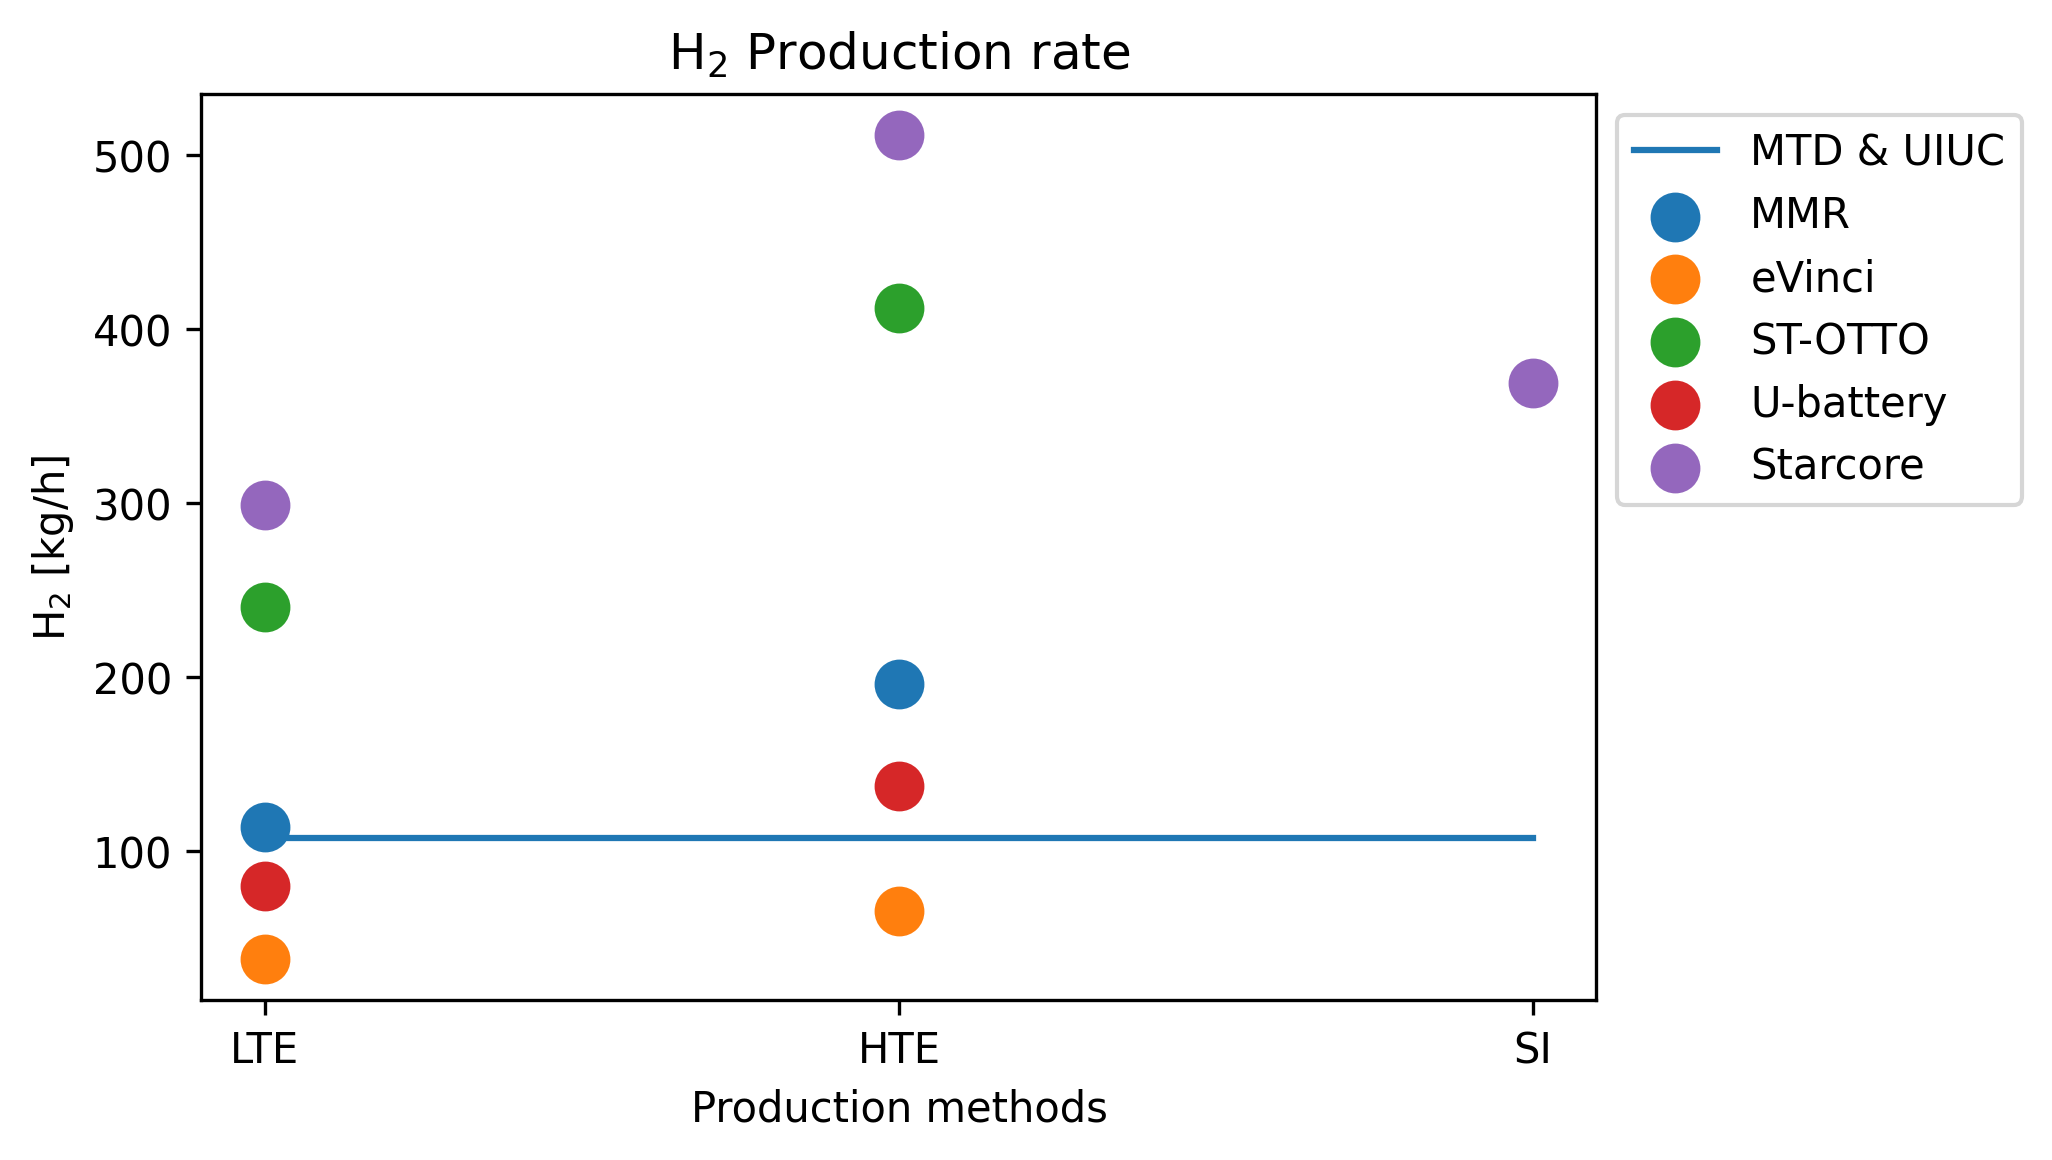
\includegraphics[height=3.8cm]{images/reactors-by-hour1}
		\end{center}
		\caption{Hydrogen production rate by the different microreactor designs.}
	\end{figure}

\end{columns}
\end{frame}

\subsection{Energy generation}
\begin{frame}
\frametitle{Net demand prediction}
\begin{columns}
    \column[t]{5cm}
	\begin{figure}[htbp!]
		\begin{center}
			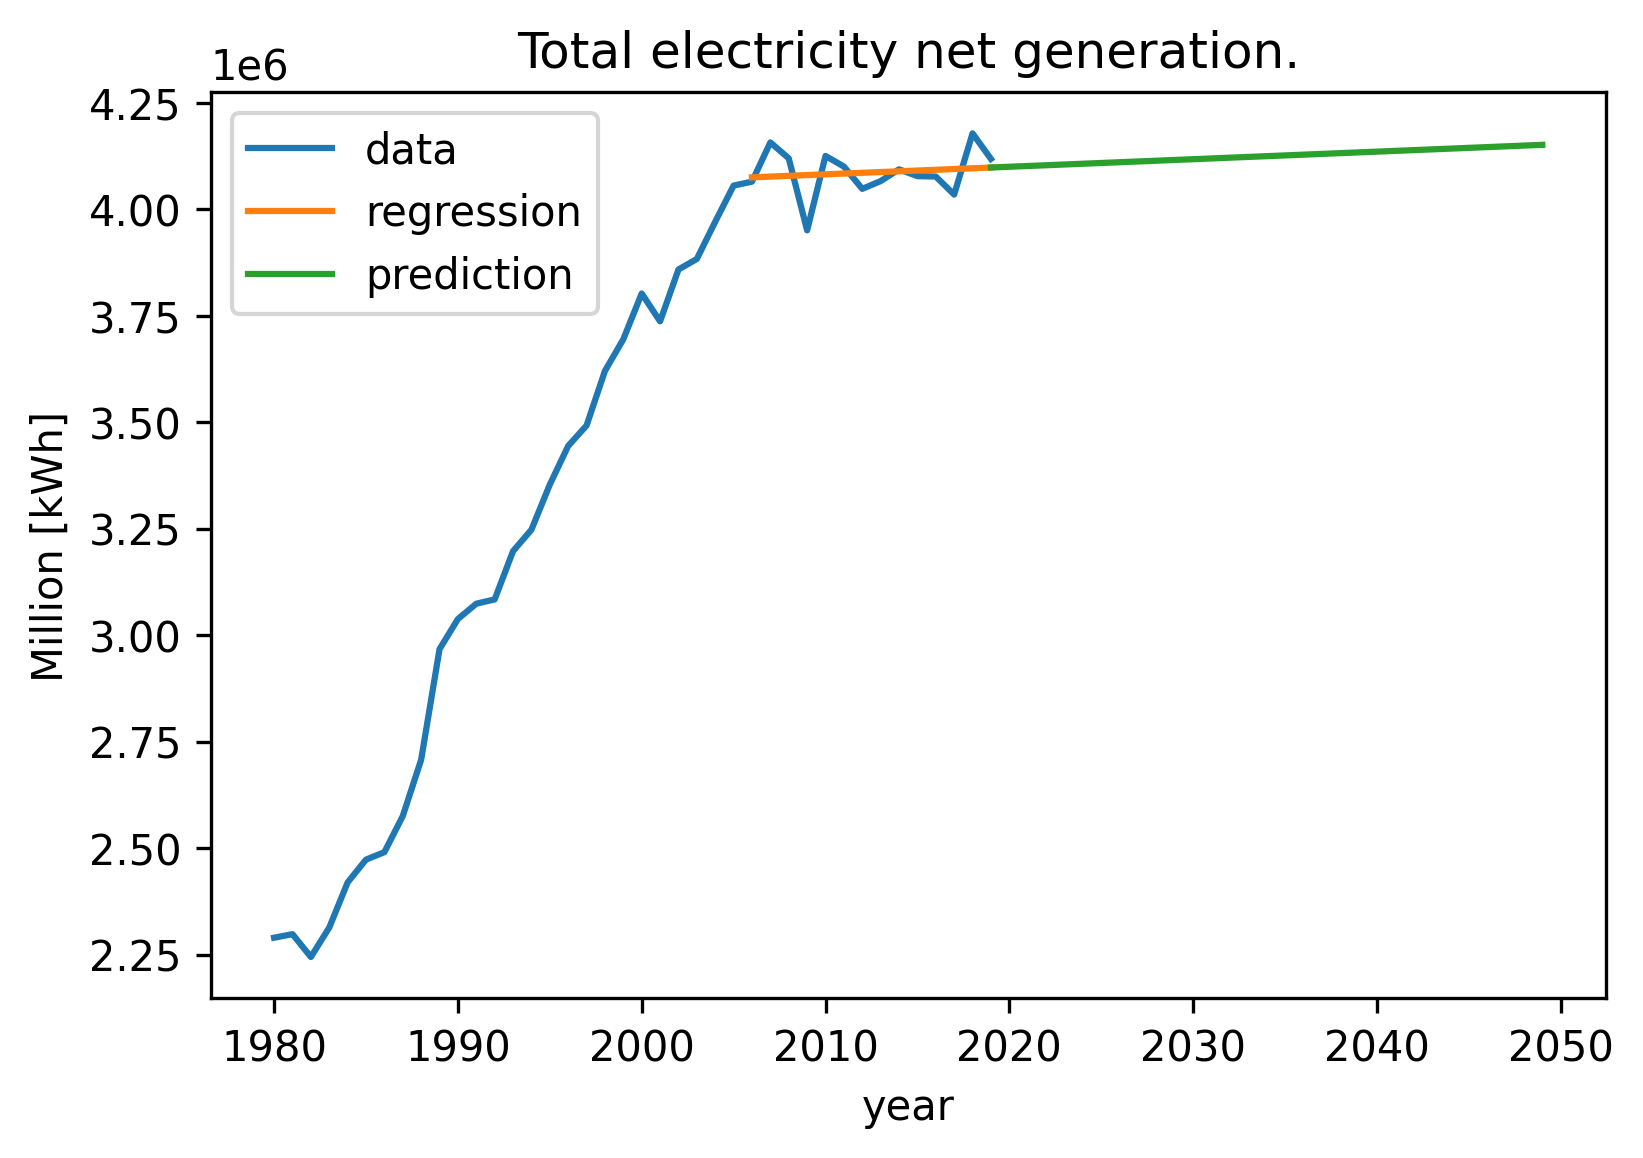
\includegraphics[height=3.3cm]{images/us-prediction1}
		\end{center}
		\caption{Prediction of the total electricity generation in the US for 2050. Data from \cite{us_energy_information_administration_electric_2020}.}
	\end{figure}

    \column[t]{5cm}
	\begin{figure}[htbp!]
		\begin{center}
			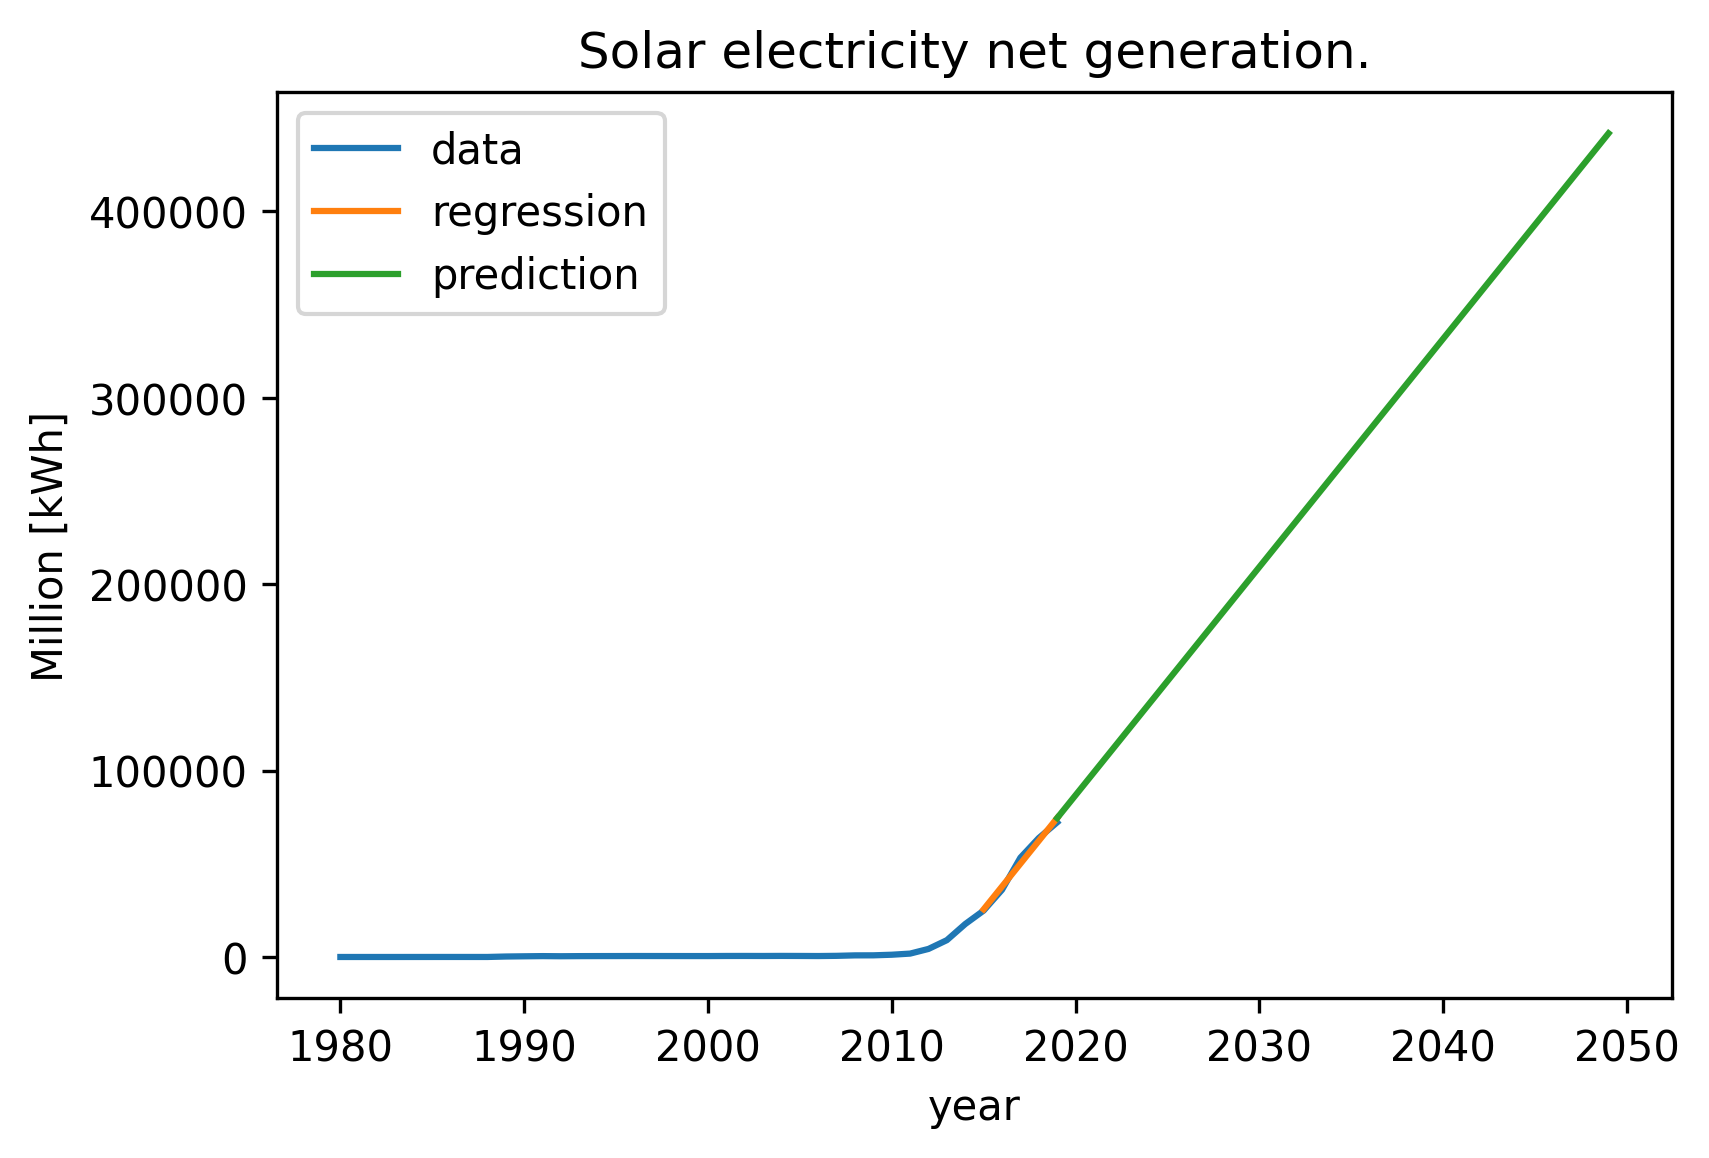
\includegraphics[height=3.3cm]{images/us-prediction2}
		\end{center}
		\caption{Prediction of the solar electricity generation in the US for 2050. Data from \cite{us_energy_information_administration_electric_2020}.}
	\end{figure}
\end{columns}
\end{frame}


\begin{frame}
\frametitle{Duck curve}
\begin{columns}
    \column[t]{5cm}
	\begin{figure}[htbp!]
		\begin{center}
			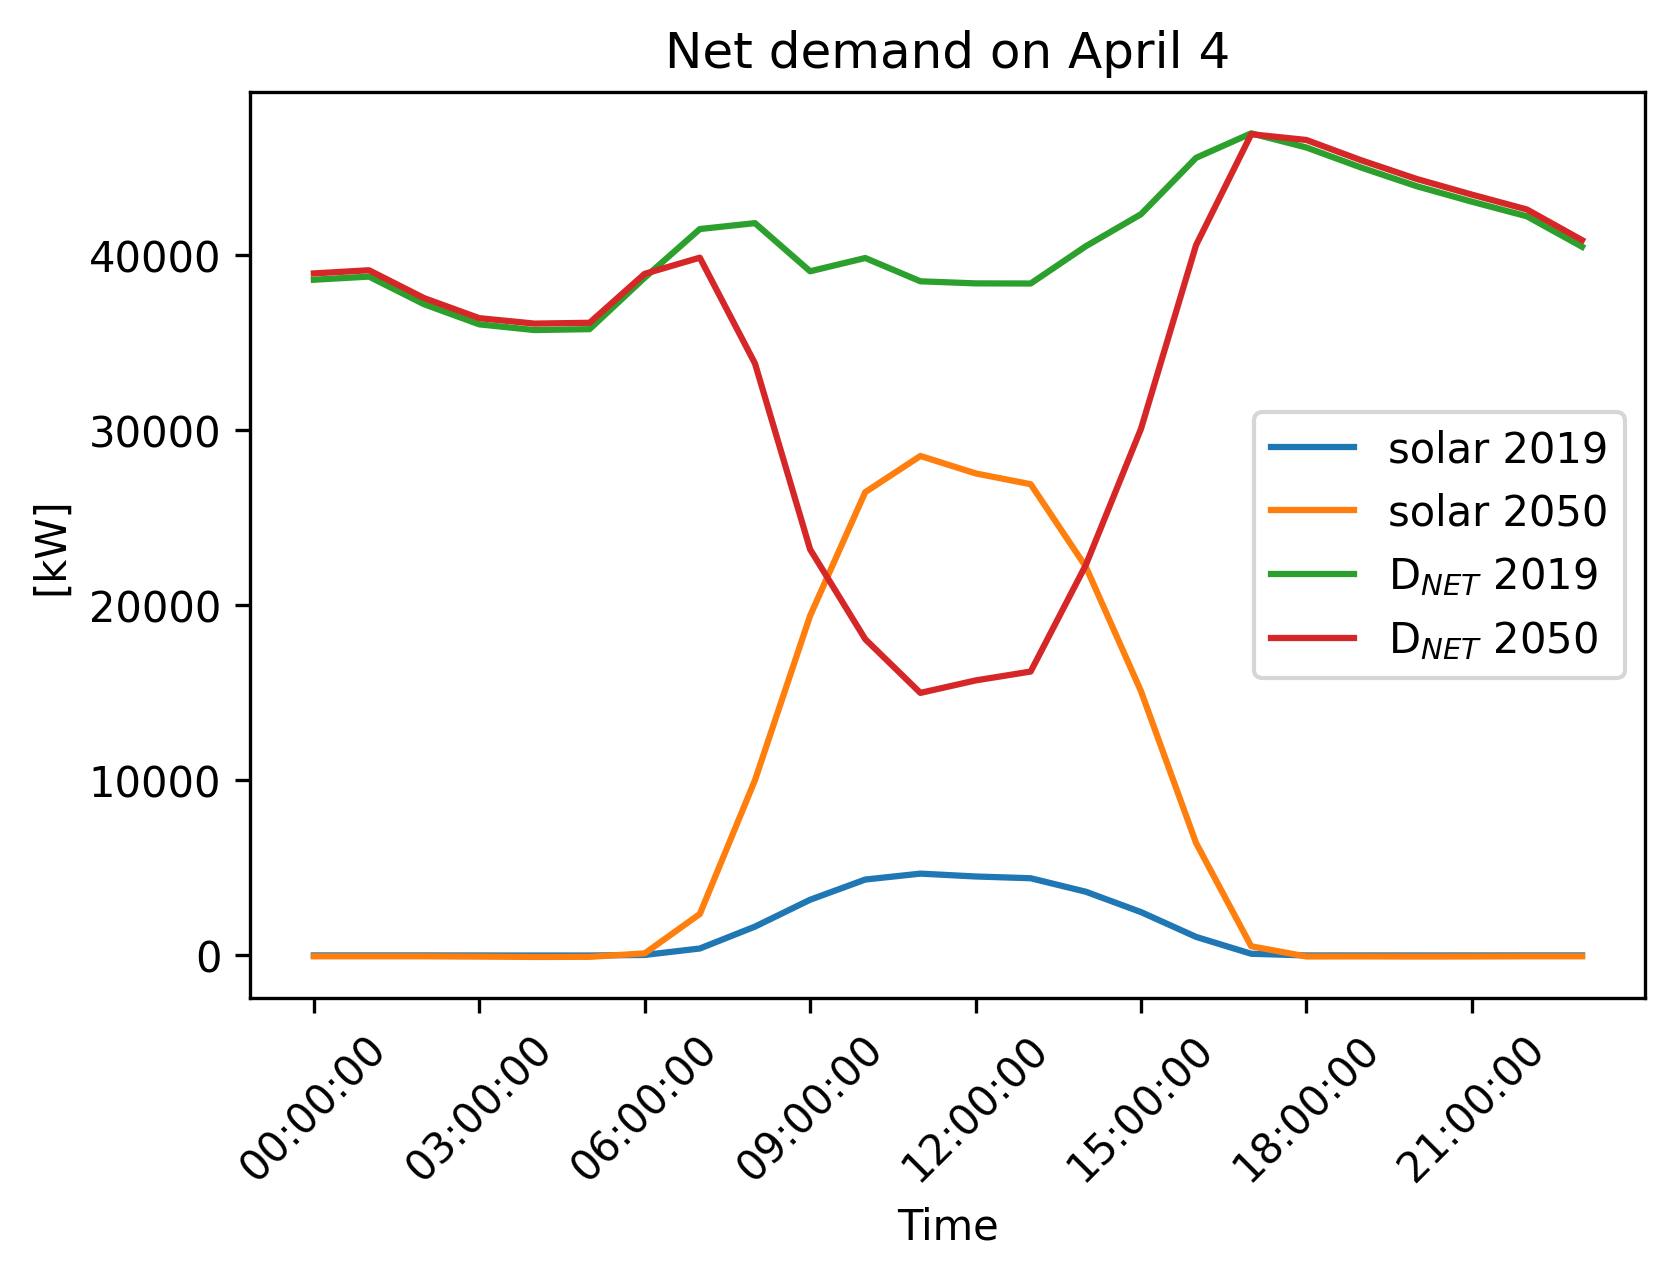
\includegraphics[height=4.0cm]{images/uiuc-duck}
		\end{center}
		\caption{Prediction of UIUC's net demand for 2050.}
	\end{figure}

    \column[t]{5.5cm}
    \begin{itemize}
 		\item Spring: solar production is higher, total demand is low.
 		\item Solar generation peaked on April 4, 2019. \vspace{0.5cm}
 	\end{itemize}

 	$D_{NET}$ = Total demand - Solar energy
	\begin{itemize}
 		\item Peak demand: 46.9 MW at 5 P.M.
 		\item Lowest demand: 15 MW at 11 A.M.
 		\item Requires an installed capacity of 31.9 MW of dispatchable sources.
 	\end{itemize}

\end{columns}
\end{frame}


\begin{frame}
\frametitle{Over-generation}
\begin{columns}
    \column[t]{5.5cm}
	\begin{figure}[htbp!]
		\begin{center}
			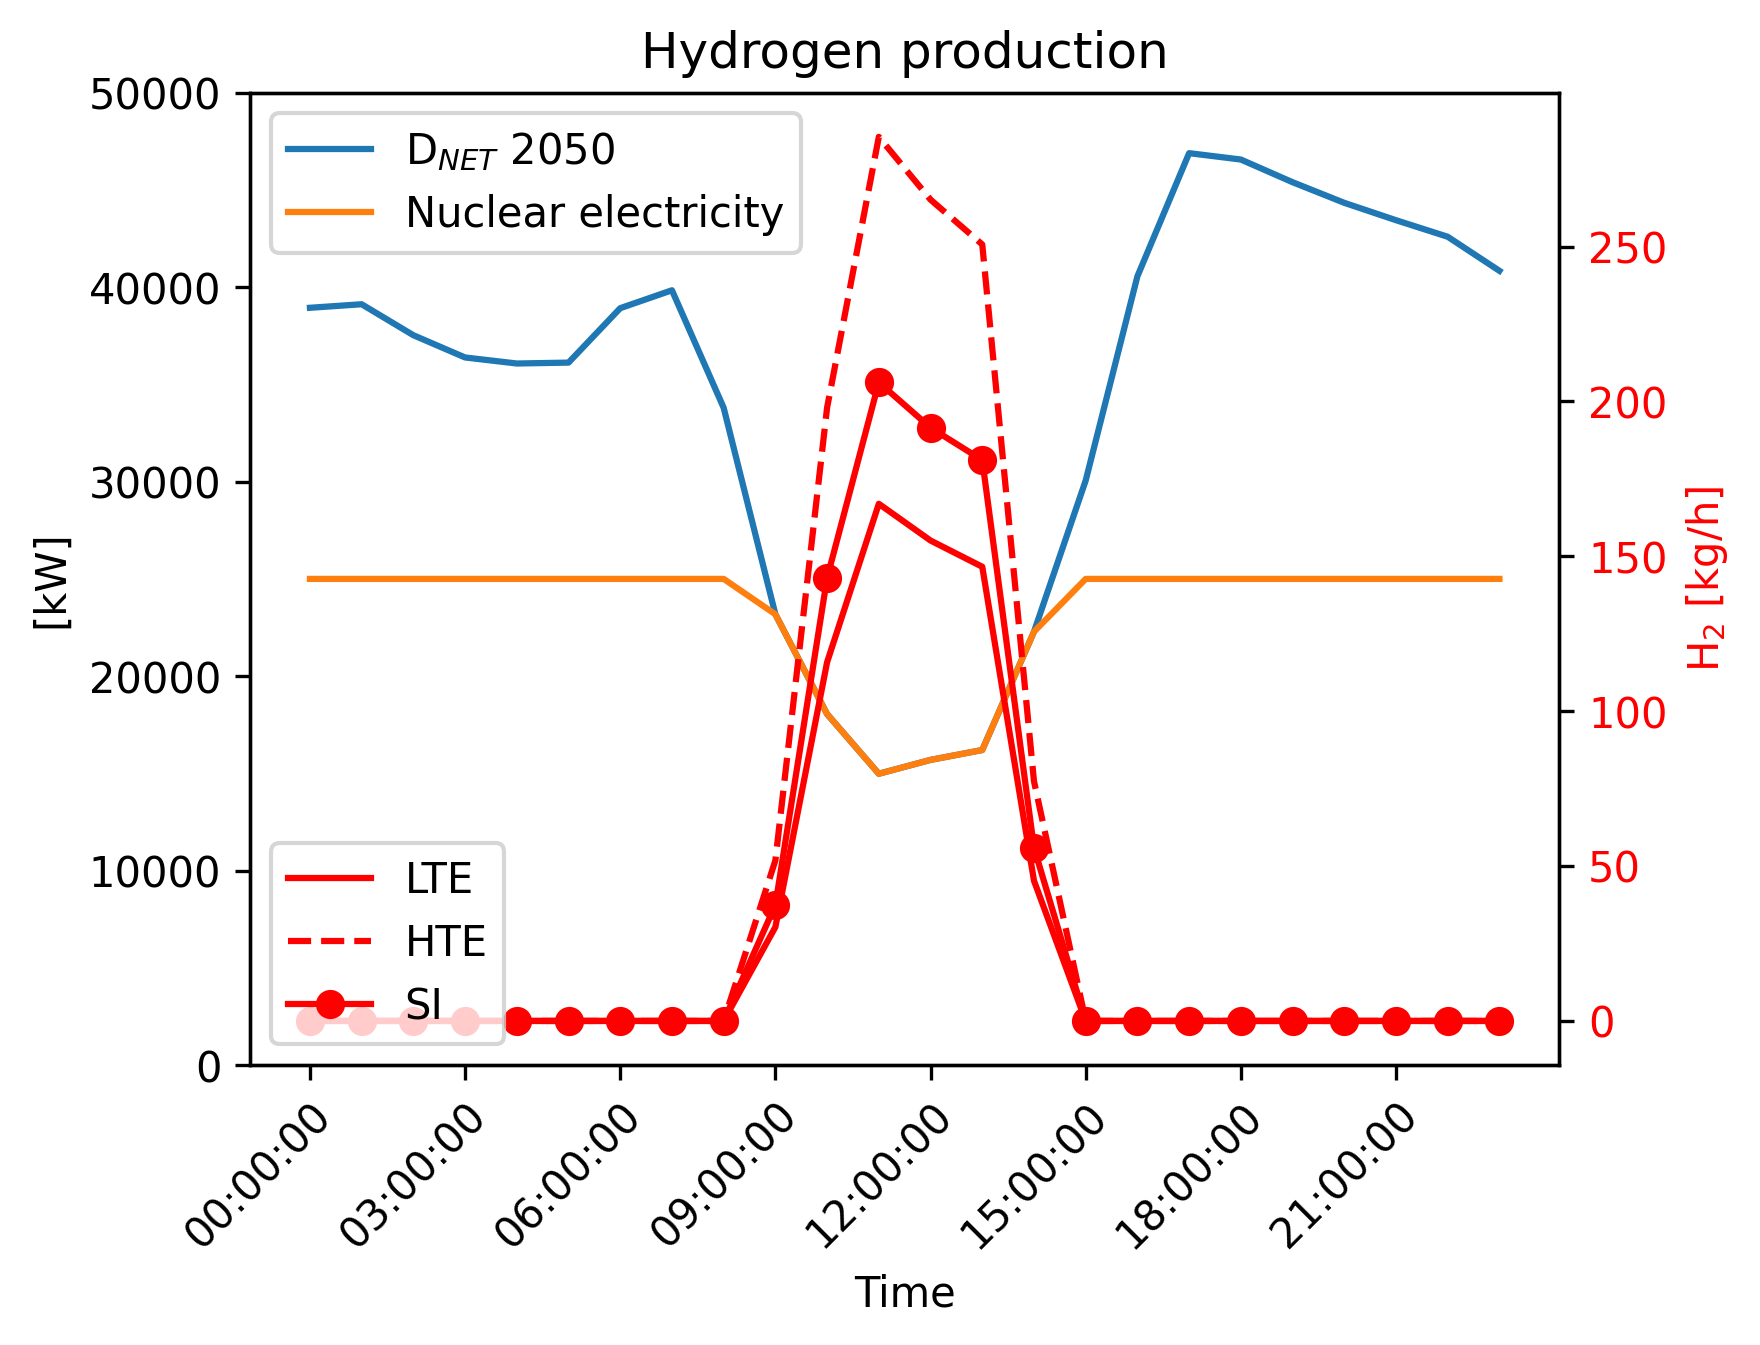
\includegraphics[height=4.4cm]{images/uiuc-hydro2B}
		\end{center}
		\caption{Hydrogen production with the excess of energy due to a net demand decrease.}
	\end{figure}

    \column[t]{5.5cm}
    \textbf{25 MWe reactor} \vspace{0.2cm}

    Low temperature electrolysis (LTE):
    \begin{itemize}
 		\item $\eta$ = 33$\%$.
 		\item Cumulative H$_2$: 660 kg.
 	\end{itemize}

    High temperature electrolysis (HTE):
    \begin{itemize}
 		\item HTGR.
 		\item T$_o$ = 850$^\circ$C.
 		\item $\eta$ = 49.8$\%$
 		\item Cumulative H$_2$: 1129 kg.
 	\end{itemize}

    Sulfur-Iodine (SI):
    \begin{itemize}
 		\item HTGR.
 		\item T$_o$ = 850$^\circ$C.
 		\item $\eta$ = 49.8$\%$
 		\item Cumulative H$_2$: 815 kg.
 	\end{itemize}

\end{columns}
\end{frame}

\begin{frame}
\frametitle{Hydrogen for energy storage}
\begin{columns}
    \column[t]{6.8cm}
	\begin{figure}[htbp!]
		\begin{center}
			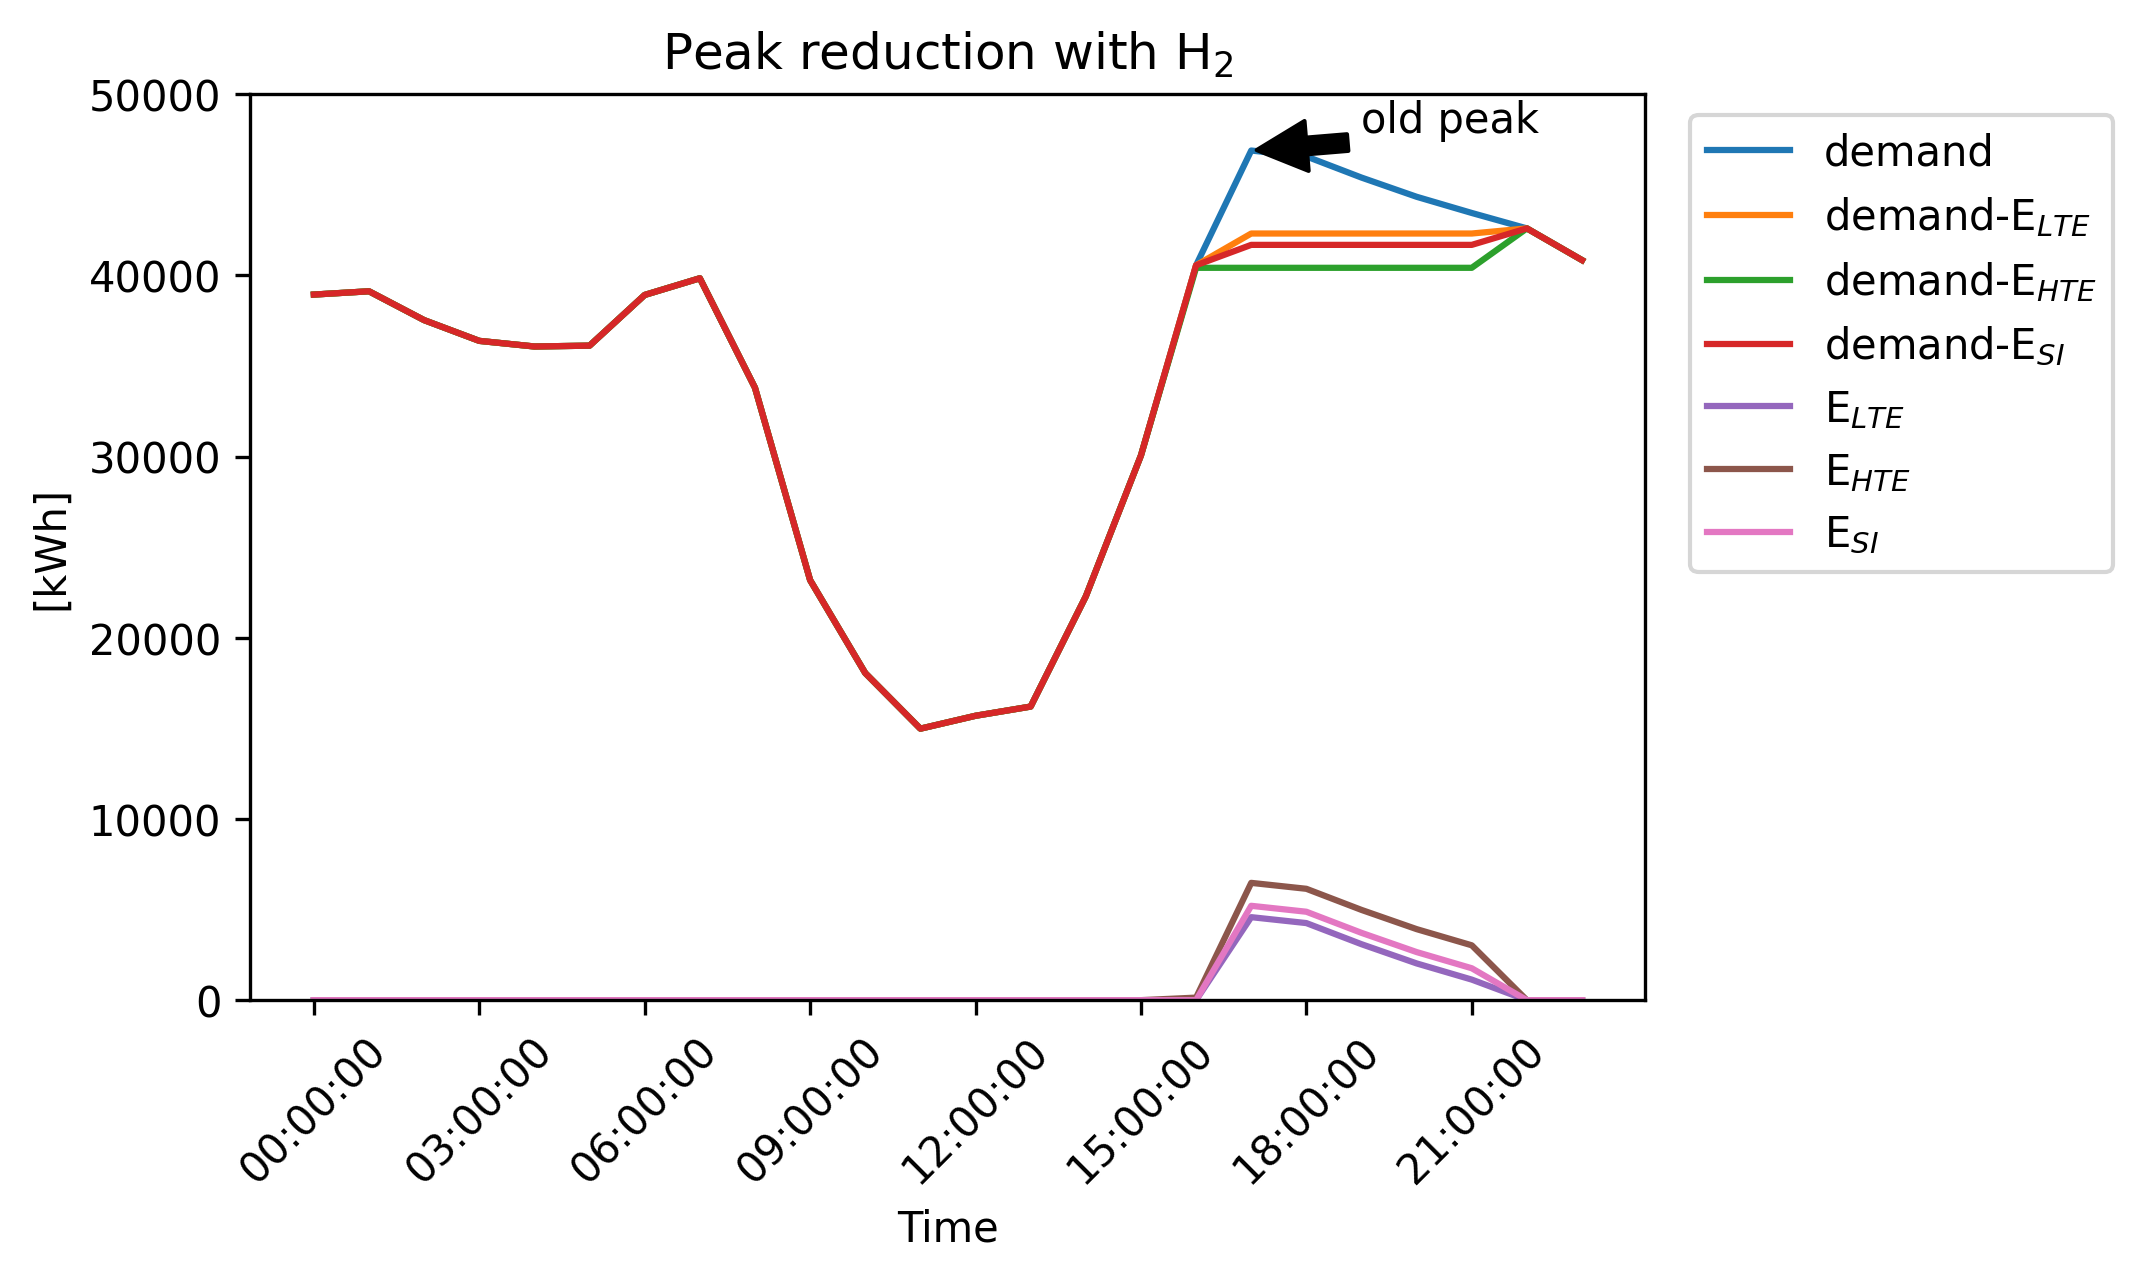
\includegraphics[height=4.2cm]{images/uiuc-hydro3B}
		\end{center}
		\caption{Peak reduction by using the produced H$_2$.}
	\end{figure}

    \column[t]{5.2cm}
    \\
    Low temperature electrolysis (LTE):
    \begin{itemize}
 		\item Electricity produced: 15.9 MWh
 		\item New peak: 41.9 MW
 		\item Peak reduction: 5 MW
 	\end{itemize}

    High temperature electrolysis (HTE):
    \begin{itemize}
		\item Electricity produced: 27.1 MWh
		\item New peak: 40.0 MW
        \item Peak reduction: 6.9 MW
 	\end{itemize}

    Sulfur-Iodine (SI):
    \begin{itemize}
		\item Electricity produced: 19.6 MWh
		\item New peak: 41.3 MW
        \item Peak reduction: 5.6 MW
 	\end{itemize}

\end{columns}
\end{frame}